\documentclass{article}
\usepackage[utf8]{inputenc}
\usepackage[italian]{babel}
\usepackage{graphicx}
\title{Sicurezza nelle reti}
\author{Giulia}
\date{\today}

\begin{document}
\maketitle

\section{Race condition}

Una Race Condition si verifica quando due o più processi/thread accedono contemporaneamente a una risorsa condivisa e il risultato finale dipende dall'ordine di esecuzione, che non è prevedibile né controllabile.

Se un programma privilegiato presenta una condizione di
competizione, gli aggressori potrebbero essere in grado di
influenzare l'output del programma privilegiato influenzando gli
eventi incontrollabili.

Quando due thread di esecuzione simultanei accedono a una risorsa
condivisa in un modo che produce involontariamente risultati diversi a
seconda della tempistica dei thread o dei processi

\begin{figure}[h]
    \centering
    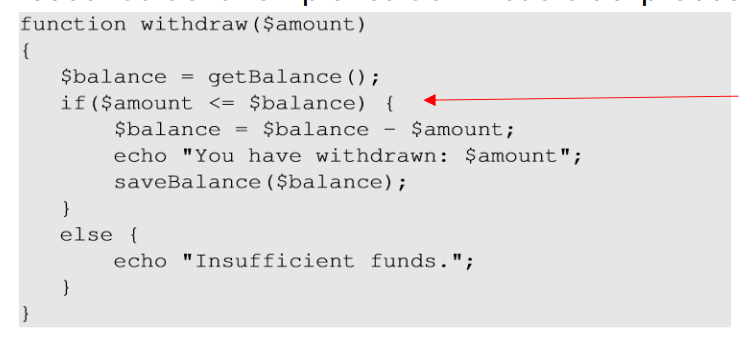
\includegraphics[width=0.6\textwidth]{immagini/1.png}
\end{figure} 
Qui può verificarsi una Race
Condition se ci sono due
richieste di prelievo
simultanee. Il controllo \texttt{if(amount <= balance)} viene superato da entrambi i thread prima che uno dei due aggiorni il saldo  (es: due richieste di prelievo simultanee di €100 su un conto con saldo di €150, primo thread getBalance() → legge 150 secondo thread getBalance() → legge 150 entrambi calcolno 150 -100 e chiamano saveBalance(50) sono stati prelevati €200, ma il saldo mostra solo €50 di differenza)


\subsection*{TOCTTOU – Time-Of-Check To Time-Of-Use}

Il TOCTTOU è un tipo speciale di Race Condition che si verifica quando intercorre un intervallo di tempo tra il momento in cui viene effettuato un controllo su una risorsa e il momento in cui quella risorsa viene effettivamente utilizzata.

Durante questa finestra temporale, un attaccante può modificare lo stato della risorsa dopo che il controllo è già avvenuto con esito positivo, ma prima che venga utilizzata. Il programma quindi opera su qualcosa di diverso da ciò che aveva verificato, con conseguenze potenzialmente gravi.

Es: un programma privilegiato controlla che un file sia sicuro, ma prima di aprirlo un attaccante lo sostituisce con un file dannoso. Il programma utilizzerà il file malevolo, credendo di aver già verificato la sua sicurezza.


Consideriamo un programma Set-UID (bit di un file eseguibile se attivato, chiunque lo lanci lo esegue con i privilegi del proprietario del file) di proprietà di root, in cui l'UID 
effettivo è root e l'ID dell'utente reale è \texttt{seed}. Il programma 
scrive in un file nella directory \texttt{/tmp}, scrivibile da tutti gli 
utenti del sistema.

l'utente seed lancia il programma, ma poiché esso è Set-UID root, il sistema operativo lo esegue come se fosse root. Quando open() apre il file, guarda l'UID effettivo (root = 0) e concede l'accesso a qualsiasi file del sistema, indipendentemente da chi lo abbia avviato.

\begin{figure}[h]
    \centering
    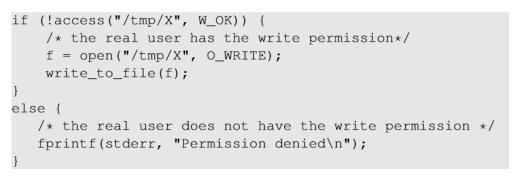
\includegraphics[width=0.6\textwidth]{immagini/2.png}
\end{figure}

Poiché root può scrivere su qualsiasi file, il programma deve prima 
verificare che sia l'utente reale ad avere i permessi necessari sul file 
di destinazione. A questo scopo viene utilizzata la funzione 
\texttt{access()}, che controlla se l'ID utente reale dispone dei 
permessi di scrittura su \texttt{/tmp/X}.

Tuttavia, tra il momento in cui \texttt{access()} effettua il controllo 
e il momento in cui \texttt{open()} apre il file in scrittura, esiste una 
finestra temporale. La funzione \texttt{open()} non controlla l'ID 
dell'utente reale, bensì quello effettivo, che è 0 (root), quindi il file 
verrà aperto indipendentemente da chi sia il proprietario effettivo del 
file in quel momento.

Un attaccante può sfruttare questa finestra temporale: dopo che 
\texttt{access()} ha verificato il file originale con esito positivo, ma 
prima che \texttt{open()} lo apra, è possibile sostituire \texttt{/tmp/X} 
con un link simbolico che punta a un file di sistema protetto, come ad 
esempio \texttt{/etc/passwd}. Il programma, eseguendosi con i privilegi 
di root, scriverà su quel file senza alcuna ulteriore verifica, 
compromettendo l'integrità del sistema.

\subsection*{Contromisure}

\begin{itemize}
	\item Operazioni atomiche : eliminare la finestra tra controllo e utilizzo
	\item Controllo e utilizzo ripetuti: per rendere difficile vincere la “gara”.
	\item Collegamento simbolico sticky anche se la directory è scrivibile da tutti, un utente può creare o eliminare solo i propri file
	\item Protezione: per impedire la creazione di collegamenti simbolici.
	\item Principi del privilegio minimo: prevenire i danni dopo che la gara è stata vinta dall'attaccante. Es. un programma non dovrebbe mantenere i privilegi di root per tutta la sua esecuzione, ma elevarli solo nel momento in cui servono e rilasciarli subito dopo.
\end{itemize}

\textbf{Operazioni atomiche}

Un primo approccio concreto utilizza i flag \texttt{O\_CREAT | O\_EXCL} 
combinati nella chiamata \texttt{open()}:

\begin{verbatim}
f = open(file, O_CREAT | O_EXCL);
\end{verbatim}

Questi due flag insieme istruiscono \texttt{open()} ad aprire il file 
solo se non esiste già: in caso contrario, l'operazione fallisce. 
Poiché controllo e apertura avvengono nella stessa chiamata di sistema, 
il kernel garantisce l'atomicità dell'intera operazione, senza lasciare 
alcuna finestra temporale sfruttabile dall'attaccante.

Un secondo approccio, puramente teorico, immagina l'esistenza di un flag 
\texttt{O\_REAL\_USER\_ID}:

\begin{verbatim}
f = open(file, O_WRITE | O_REAL_USER_ID);
\end{verbatim}

Questo flag istruirebbe \texttt{open()} a verificare i permessi 
utilizzando l'UID reale anziché quello effettivo, affidando a una singola 
chiamata sia il controllo che l'utilizzo. 

\textbf{Controllo e utilizzo ripetuti}

Un secondo approccio consiste nel ripetere più volte la sequenza di 
controllo e utilizzo all'interno dello stesso programma. Come mostrato 
nel codice, il ciclo \texttt{access()} e \texttt{open()} viene eseguito 
tre volte, producendo tre file descriptor \texttt{fd1}, \texttt{fd2} e 
\texttt{fd3}. Al termine, il programma verifica tramite \texttt{fstat()} 
che i tre file descriptor puntino allo stesso inode:

\begin{figure}[h]
    \centering
    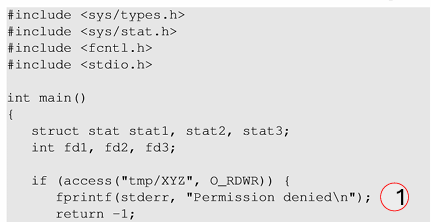
\includegraphics[width=0.6\textwidth]{immagini/3.png}
\end{figure}

\begin{figure}[h]
    \centering
    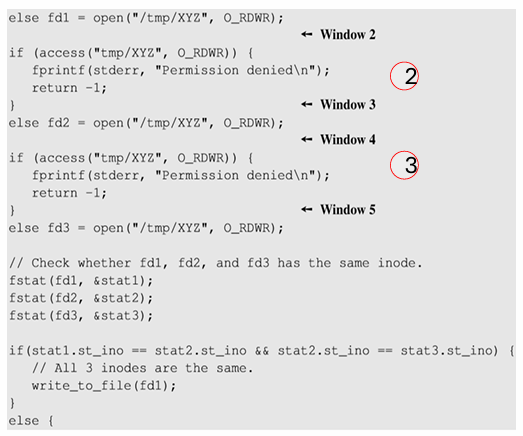
\includegraphics[width=0.6\textwidth]{immagini/4.png}
\end{figure}


\begin{verbatim}
if(stat1.st_ino == stat2.st_ino && stat2.st_ino == stat3.st_ino) {
    write_to_file(fd1);
}
\end{verbatim}

Se gli inode non coincidono, significa che il file è stato modificato 
durante l'esecuzione e l'operazione viene bloccata. Per portare a termine 
un attacco riuscito, l'attaccante dovrebbe riuscire a sostituire 
\texttt{/tmp/XYZ} esattamente in ognuna delle cinque finestre temporali 
disponibili tra i vari controlli e aperture. La probabilità di riuscire 
a vincere la gara cinque volte consecutive è drasticamente inferiore 
rispetto a un programma con una sola condizione di competizione. Questa 
contromisura non elimina teoricamente la vulnerabilità, ma la rende 
nella pratica estremamente difficile da sfruttare.

\textbf{Protezione permanente dei collegamenti simbolici}

I sistemi Linux moderni offrono una protezione permanente contro l'abuso 
dei collegamenti simbolici nelle directory scrivibili da tutti, come 
\texttt{/tmp}. Quando questa protezione è abilitata, un collegamento 
simbolico all'interno di una directory scrivibile da tutti può essere 
seguito solo se il proprietario del collegamento coincide con l'utente 
che lo sta seguendo, oppure con il proprietario della directory stessa. 
Questo impedisce all'attaccante di creare un link simbolico malevolo 
che punti a file di sistema protetti, poiché il programma privilegiato 
non sarà autorizzato a seguirlo.

\begin{figure}[h]
    \centering
    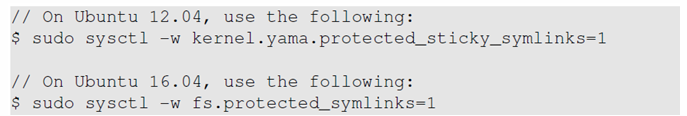
\includegraphics[width=0.6\textwidth]{immagini/5.png}
\end{figure}



\end{document}